\documentclass[final]{beamer} % beamer 3.10: do NOT use option hyperref={pdfpagelabels=false} !
%\documentclass[final,hyperref={pdfpagelabels=false}]{beamer} % beamer 3.07: get rid of beamer warnings
\mode<presentation> {  %% check http://www-i6.informatik.rwth-aachen.de/~dreuw/latexbeamerposter.php for examples
  \usetheme{qcv}    %% you should define your own theme e.g. for big headlines using your own logos 
}
\usepackage[english]{babel}
\usepackage[latin1]{inputenc}
\usepackage{amsmath,amsthm, amssymb, latexsym}
%\usepackage{times}\usefonttheme{professionalfonts}  % times is obsolete
\usefonttheme[onlymath]{serif}
\boldmath
\usepackage[orientation=landscape,size=a0,scale=1.4,debug]{beamerposter}                       % e.g. for DIN-A0 poster
%\usepackage[orientation=portrait,size=a1,scale=1.4,grid,debug]{beamerposter}                  % e.g. for DIN-A1 poster, with optional grid and debug output
%\usepackage[size=custom,width=200,height=120,scale=2,debug]{beamerposter}                     % e.g. for custom size poster
%\usepackage[orientation=portrait,size=a0,scale=1.0,printer=rwth-glossy-uv.df]{beamerposter}   % e.g. for DIN-A0 poster with rwth-glossy-uv printer check

\title[QCViewer]{QCViewer}
\author[Author]{Author and Author}
\institute[IQC, University of Waterloo]{Quantum Circuits group, IQC, University of Waterloo}
\date{\today}


\begin{document}
  \begin{frame}{} 
  \begin{columns}
    \begin{column}{.33\textwidth}
      \begin{beamercolorbox}[center,wd=\textwidth]{postercolumn}
         \begin{minipage}[T]{.95\textwidth}
           \begin{block}{\large Overview}
             QCViewer is a tool for displaying, editing, and simulating quantum circuits.

             \centering 
             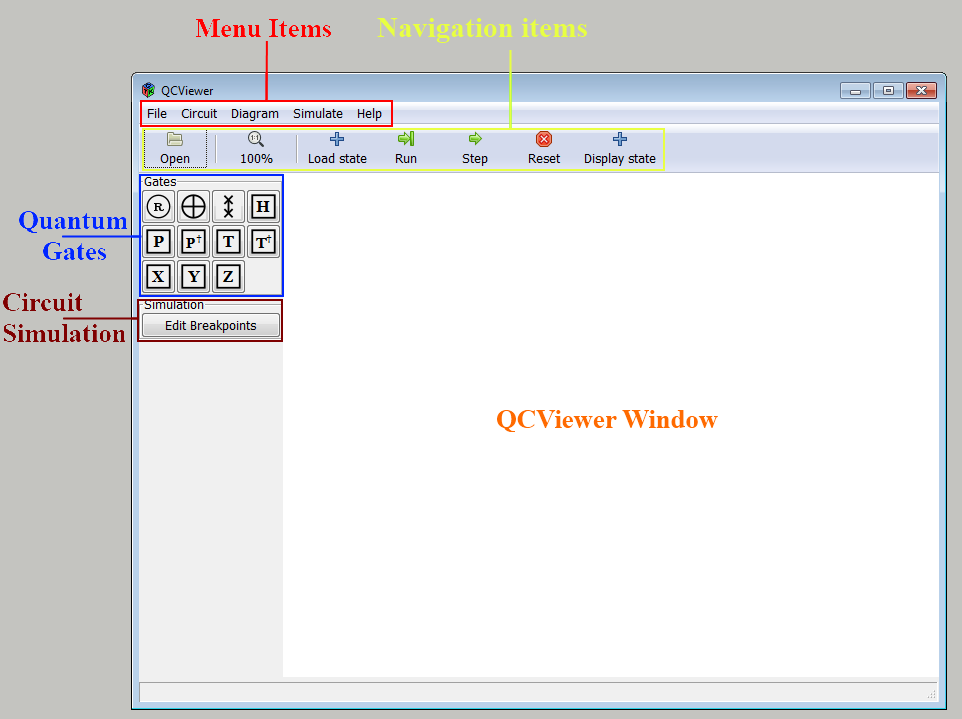
\includegraphics{figures/QCViewerGUI.png}
           \end{block}
           \begin{block}{\large Motivation}
             In creating QCViewer, our goal was to develop a convenient tool that would be useful to 
             the quantum computing community for both research and educational purposes. 

             QCViewer provides a drag and drop interface for circuit design. This makes it easy to quickly 
             test out new algorithm and circuit design ideas. In order to make the diagrams useful for presentation 
             (e.g., Adobe Illustrator, PowerPoint) and publication (e.g., LaTex) we provide the ability to export 
             images in scalabe vector graphics (.svg) and portable network graphics (.png).
           \end{block}
         \end{minipage}
      \end{beamercolorbox}
    \end{column}
    \begin{column}{.33\textwidth}
      \begin{beamercolorbox}[center,wd=\textwidth]{postercolumn}
         \begin{minipage}[T]{.95\textwidth}
           \begin{block}{\large Circuit Design}
             Circuits can be designed on screen with drag and drop or by writting a .qc circuit file.
           \end{block}
         \end{minipage}
      \end{beamercolorbox}
    \end{column}
    \begin{column}{.33\textwidth}
      \begin{beamercolorbox}[center,wd=\textwidth]{postercolumn}
         \begin{minipage}[T]{.95\textwidth}
           \begin{block}{\large Circuit Simulation}
              Our circuit simulator is state-vector based.
           \end{block}
         \end{minipage}
      \end{beamercolorbox}
    \end{column}
  \end{columns}
  \end{frame}
\end{document}
